%% FreqODES -- journal manuscript, Elsevier CAS double-column template (cas-dc)
%% Compile: pdflatex main && bibtex main && pdflatex main && pdflatex main   (or Overleaf, "Elsevier CAS Double Column")
\documentclass[a4paper,fleqn]{cas-dc}
\usepackage[T1]{fontenc}
\usepackage{lmodern}
\usepackage[numbers,sort&compress]{natbib}
\usepackage{booktabs,multirow,graphicx,amsmath,xcolor}
\usepackage{tikz}
\usepackage{algorithm}
\usepackage{algpseudocode}
\usetikzlibrary{arrows.meta,positioning,fit,backgrounds}

% Remove the template's left footer ("<short authors>: Preprint submitted to Elsevier"); keep "Page x of y"
\ExplSyntaxOn
\cs_set:Npn \__first_footerline: {}
\ExplSyntaxOff

\newcommand{\DFUSEDKTenLThreeQ}{78.93}
\newcommand{\JFUSEDKTenLThreeQ}{66.22}
\newcommand{\TFUSEDKTenLThreeQ}{169}
\newcommand{\DFUSEDKTenLThreeQLiver}{87.04}
\newcommand{\JFUSEDKTenLThreeQLiver}{77.66}
\newcommand{\DFUSEDKTenLThreeQLK}{75.32}
\newcommand{\JFUSEDKTenLThreeQLK}{61.16}
\newcommand{\DFUSEDKTenLThreeQRK}{74.58}
\newcommand{\JFUSEDKTenLThreeQRK}{60.08}
\newcommand{\DFUSEDKTenLThreeQSpleen}{78.79}
\newcommand{\JFUSEDKTenLThreeQSpleen}{65.96}
\newcommand{\DBNKTennoDW}{78.73}
\newcommand{\JBNKTennoDW}{66.05}
\newcommand{\TBNKTennoDW}{166}
\newcommand{\DBNKTennoDWLiver}{87.26}
\newcommand{\JBNKTennoDWLiver}{77.90}
\newcommand{\DBNKTennoDWLK}{75.33}
\newcommand{\JBNKTennoDWLK}{61.33}
\newcommand{\DBNKTennoDWRK}{74.02}
\newcommand{\JBNKTennoDWRK}{59.46}
\newcommand{\DBNKTennoDWSpleen}{78.31}
\newcommand{\JBNKTennoDWSpleen}{65.49}
\newcommand{\DFUSEDKTenLFifty}{78.40}
\newcommand{\JFUSEDKTenLFifty}{65.45}
\newcommand{\TFUSEDKTenLFifty}{169}
\newcommand{\DFUSEDKTenLFiftyLiver}{86.11}
\newcommand{\JFUSEDKTenLFiftyLiver}{76.16}
\newcommand{\DFUSEDKTenLFiftyLK}{75.22}
\newcommand{\JFUSEDKTenLFiftyLK}{61.05}
\newcommand{\DFUSEDKTenLFiftyRK}{74.15}
\newcommand{\JFUSEDKTenLFiftyRK}{59.48}
\newcommand{\DFUSEDKTenLFiftySpleen}{78.12}
\newcommand{\JFUSEDKTenLFiftySpleen}{65.12}
\newcommand{\DBNKTen}{78.83}
\newcommand{\JBNKTen}{66.24}
\newcommand{\TBNKTen}{167}
\newcommand{\DBNKTenLiver}{87.88}
\newcommand{\JBNKTenLiver}{78.79}
\newcommand{\DBNKTenLK}{75.19}
\newcommand{\JBNKTenLK}{61.21}
\newcommand{\DBNKTenRK}{74.18}
\newcommand{\JBNKTenRK}{59.65}
\newcommand{\DBNKTenSpleen}{78.06}
\newcommand{\JBNKTenSpleen}{65.31}
\newcommand{\DFUSEDKTenLQuarter}{79.09}
\newcommand{\JFUSEDKTenLQuarter}{66.37}
\newcommand{\TFUSEDKTenLQuarter}{168}
\newcommand{\DFUSEDKTenLQuarterLiver}{87.63}
\newcommand{\JFUSEDKTenLQuarterLiver}{78.41}
\newcommand{\DFUSEDKTenLQuarterLK}{75.54}
\newcommand{\JFUSEDKTenLQuarterLK}{61.28}
\newcommand{\DFUSEDKTenLQuarterRK}{74.18}
\newcommand{\JFUSEDKTenLQuarterRK}{59.65}
\newcommand{\DFUSEDKTenLQuarterSpleen}{79.01}
\newcommand{\JFUSEDKTenLQuarterSpleen}{66.16}
\newcommand{\DFREQKTen}{78.20}
\newcommand{\JFREQKTen}{65.27}
\newcommand{\TFREQKTen}{109}
\newcommand{\DFREQKTenLiver}{87.28}
\newcommand{\JFREQKTenLiver}{77.80}
\newcommand{\DFREQKTenLK}{74.31}
\newcommand{\JFREQKTenLK}{59.92}
\newcommand{\DFREQKTenRK}{73.46}
\newcommand{\JFREQKTenRK}{58.76}
\newcommand{\DFREQKTenSpleen}{77.74}
\newcommand{\JFREQKTenSpleen}{64.59}
\newcommand{\DDWTKTen}{78.15}
\newcommand{\JDWTKTen}{65.28}
\newcommand{\TDWTKTen}{109}
\newcommand{\DDWTKTenLiver}{87.45}
\newcommand{\JDWTKTenLiver}{78.13}
\newcommand{\DDWTKTenLK}{74.00}
\newcommand{\JDWTKTenLK}{59.62}
\newcommand{\DDWTKTenRK}{73.31}
\newcommand{\JDWTKTenRK}{58.59}
\newcommand{\DDWTKTenSpleen}{77.84}
\newcommand{\JDWTKTenSpleen}{64.77}
\newcommand{\DRANDOMKFifty}{79.52}
\newcommand{\JRANDOMKFifty}{67.00}
\newcommand{\TRANDOMKFifty}{113}
\newcommand{\DRANDOMKFiftyLiver}{87.81}
\newcommand{\JRANDOMKFiftyLiver}{78.54}
\newcommand{\DRANDOMKFiftyLK}{77.41}
\newcommand{\JRANDOMKFiftyLK}{63.76}
\newcommand{\DRANDOMKFiftyRK}{75.26}
\newcommand{\JRANDOMKFiftyRK}{60.85}
\newcommand{\DRANDOMKFiftySpleen}{77.59}
\newcommand{\JRANDOMKFiftySpleen}{64.84}
\newcommand{\DBNKFifty}{79.57}
\newcommand{\JBNKFifty}{67.00}
\newcommand{\TBNKFifty}{171}
\newcommand{\DBNKFiftyLiver}{88.02}
\newcommand{\JBNKFiftyLiver}{78.88}
\newcommand{\DBNKFiftyLK}{76.66}
\newcommand{\JBNKFiftyLK}{62.74}
\newcommand{\DBNKFiftyRK}{75.71}
\newcommand{\JBNKFiftyRK}{61.40}
\newcommand{\DBNKFiftySpleen}{77.89}
\newcommand{\JBNKFiftySpleen}{64.96}
\newcommand{\DRANDOMKTennoDW}{78.96}
\newcommand{\JRANDOMKTennoDW}{66.29}
\newcommand{\TRANDOMKTennoDW}{109}
\newcommand{\DRANDOMKTennoDWLiver}{87.98}
\newcommand{\JRANDOMKTennoDWLiver}{78.81}
\newcommand{\DRANDOMKTennoDWLK}{75.29}
\newcommand{\JRANDOMKTennoDWLK}{61.07}
\newcommand{\DRANDOMKTennoDWRK}{74.27}
\newcommand{\JRANDOMKTennoDWRK}{59.74}
\newcommand{\DRANDOMKTennoDWSpleen}{78.31}
\newcommand{\JRANDOMKTennoDWSpleen}{65.55}
\newcommand{\DFFTKFifty}{79.24}
\newcommand{\JFFTKFifty}{66.61}
\newcommand{\TFFTKFifty}{115}
\newcommand{\DFFTKFiftyLiver}{88.08}
\newcommand{\JFFTKFiftyLiver}{78.95}
\newcommand{\DFFTKFiftyLK}{76.43}
\newcommand{\JFFTKFiftyLK}{62.50}
\newcommand{\DFFTKFiftyRK}{75.08}
\newcommand{\JFFTKFiftyRK}{60.61}
\newcommand{\DFFTKFiftySpleen}{77.37}
\newcommand{\JFFTKFiftySpleen}{64.38}
\newcommand{\DFFTKTen}{78.02}
\newcommand{\JFFTKTen}{65.03}
\newcommand{\TFFTKTen}{107}
\newcommand{\DFFTKTenLiver}{87.43}
\newcommand{\JFFTKTenLiver}{77.94}
\newcommand{\DFFTKTenLK}{73.65}
\newcommand{\JFFTKTenLK}{59.12}
\newcommand{\DFFTKTenRK}{73.59}
\newcommand{\JFFTKTenRK}{58.83}
\newcommand{\DFFTKTenSpleen}{77.41}
\newcommand{\JFFTKTenSpleen}{64.22}
\newcommand{\DFREQKFifty}{79.20}
\newcommand{\JFREQKFifty}{66.52}
\newcommand{\TFREQKFifty}{114}
\newcommand{\DFREQKFiftyLiver}{87.84}
\newcommand{\JFREQKFiftyLiver}{78.60}
\newcommand{\DFREQKFiftyLK}{76.38}
\newcommand{\JFREQKFiftyLK}{62.44}
\newcommand{\DFREQKFiftyRK}{74.79}
\newcommand{\JFREQKFiftyRK}{60.24}
\newcommand{\DFREQKFiftySpleen}{77.80}
\newcommand{\JFREQKFiftySpleen}{64.82}
\newcommand{\DODESK}{79.52}
\newcommand{\JODESK}{66.96}
\newcommand{\TODESK}{117}
\newcommand{\DODESKLiver}{87.89}
\newcommand{\JODESKLiver}{78.69}
\newcommand{\DODESKLK}{76.90}
\newcommand{\JODESKLK}{63.10}
\newcommand{\DODESKRK}{75.28}
\newcommand{\JODESKRK}{60.86}
\newcommand{\DODESKSpleen}{78.00}
\newcommand{\JODESKSpleen}{65.19}
\newcommand{\Dsourceonly}{54.97}
\newcommand{\Jsourceonly}{42.74}
\newcommand{\Tsourceonly}{49}
\newcommand{\DsourceonlyLiver}{85.89}
\newcommand{\JsourceonlyLiver}{75.60}
\newcommand{\DsourceonlyLK}{29.84}
\newcommand{\JsourceonlyLK}{18.21}
\newcommand{\DsourceonlyRK}{33.74}
\newcommand{\JsourceonlyRK}{21.79}
\newcommand{\DsourceonlySpleen}{70.43}
\newcommand{\JsourceonlySpleen}{55.38}
\newcommand{\DFUSEDKFiftyLFifty}{79.50}
\newcommand{\JFUSEDKFiftyLFifty}{66.92}
\newcommand{\TFUSEDKFiftyLFifty}{173}
\newcommand{\DFUSEDKFiftyLFiftyLiver}{88.04}
\newcommand{\JFUSEDKFiftyLFiftyLiver}{78.91}
\newcommand{\DFUSEDKFiftyLFiftyLK}{76.70}
\newcommand{\JFUSEDKFiftyLFiftyLK}{62.91}
\newcommand{\DFUSEDKFiftyLFiftyRK}{75.27}
\newcommand{\JFUSEDKFiftyLFiftyRK}{60.83}
\newcommand{\DFUSEDKFiftyLFiftySpleen}{77.99}
\newcommand{\JFUSEDKFiftyLFiftySpleen}{65.04}
\newcommand{\DRANDOMKTen}{78.75}
\newcommand{\JRANDOMKTen}{66.04}
\newcommand{\TRANDOMKTen}{107}
\newcommand{\DRANDOMKTenLiver}{88.11}
\newcommand{\JRANDOMKTenLiver}{78.96}
\newcommand{\DRANDOMKTenLK}{75.80}
\newcommand{\JRANDOMKTenLK}{61.62}
\newcommand{\DRANDOMKTenRK}{74.34}
\newcommand{\JRANDOMKTenRK}{59.79}
\newcommand{\DRANDOMKTenSpleen}{76.75}
\newcommand{\JRANDOMKTenSpleen}{63.77}
\newcommand{\DFREQKTennoDW}{78.32}
\newcommand{\JFREQKTennoDW}{65.42}
\newcommand{\TFREQKTennoDW}{110}
\newcommand{\DFREQKTennoDWLiver}{87.35}
\newcommand{\JFREQKTennoDWLiver}{77.92}
\newcommand{\DFREQKTennoDWLK}{74.53}
\newcommand{\JFREQKTennoDWLK}{60.18}
\newcommand{\DFREQKTennoDWRK}{73.40}
\newcommand{\JFREQKTennoDWRK}{58.71}
\newcommand{\DFREQKTennoDWSpleen}{78.00}
\newcommand{\JFREQKTennoDWSpleen}{64.87}
\newcommand{\DDWTKFifty}{79.09}
\newcommand{\JDWTKFifty}{66.43}
\newcommand{\TDWTKFifty}{114}
\newcommand{\DDWTKFiftyLiver}{87.97}
\newcommand{\JDWTKFiftyLiver}{78.80}
\newcommand{\DDWTKFiftyLK}{76.35}
\newcommand{\JDWTKFiftyLK}{62.43}
\newcommand{\DDWTKFiftyRK}{74.62}
\newcommand{\JDWTKFiftyRK}{60.10}
\newcommand{\DDWTKFiftySpleen}{77.41}
\newcommand{\JDWTKFiftySpleen}{64.39}
\newcommand{\PFFTKTen}{0.005}
\newcommand{\DiffFFTKTen}{-0.81}
\newcommand{\PDWTKTen}{0.027}
\newcommand{\DiffDWTKTen}{-0.67}
\newcommand{\PFREQKTen}{0.091}
\newcommand{\DiffFREQKTen}{-0.63}
\newcommand{\PFUSEDKTenLFifty}{0.159}
\newcommand{\DiffFUSEDKTenLFifty}{-0.43}
\newcommand{\PRANDOMKTen}{0.334}
\newcommand{\DiffRANDOMKTen}{-0.08}
\newcommand{\PFFTKFifty}{0.064}
\newcommand{\DiffFFTKFifty}{-0.33}
\newcommand{\PDWTKFifty}{0.030}
\newcommand{\DiffDWTKFifty}{-0.48}
\newcommand{\PFREQKFifty}{0.044}
\newcommand{\DiffFREQKFifty}{-0.37}
\newcommand{\PFUSEDKFiftyLFifty}{0.687}
\newcommand{\DiffFUSEDKFiftyLFifty}{-0.07}
\newcommand{\PRANDOMKFifty}{1.000}
\newcommand{\DiffRANDOMKFifty}{-0.05}
\newcommand{\AUCFFT}{0.994}
\newcommand{\AUCDWT}{0.969}
\newcommand{\AUCFREQ}{0.993}
     % single-seed results (make_report.py)
\newcommand{\VBnTenMean}{78.31}
\newcommand{\VBnTenStd}{1.38}
\newcommand{\VBnTenDiff}{+0.00}
\newcommand{\VBnTenP}{1.000}
\newcommand{\VBnTenIoU}{65.51}
\newcommand{\VBnTenTime}{154}
\newcommand{\VBnTenSa}{76.80}
\newcommand{\VBnTenSb}{78.67}
\newcommand{\VBnTenSc}{79.48}
\newcommand{\VFqTenMean}{78.54}
\newcommand{\VFqTenStd}{0.13}
\newcommand{\VFqTenDiff}{+0.22}
\newcommand{\VFqTenP}{0.908}
\newcommand{\VFqTenIoU}{65.63}
\newcommand{\VFqTenTime}{104}
\newcommand{\VFqTenSa}{78.39}
\newcommand{\VFqTenSb}{78.62}
\newcommand{\VFqTenSc}{78.61}
\newcommand{\VFvTenMean}{78.66}
\newcommand{\VFvTenStd}{0.26}
\newcommand{\VFvTenDiff}{+0.35}
\newcommand{\VFvTenP}{0.199}
\newcommand{\VFvTenIoU}{65.84}
\newcommand{\VFvTenTime}{105}
\newcommand{\VFvTenSa}{78.36}
\newcommand{\VFvTenSb}{78.80}
\newcommand{\VFvTenSc}{78.82}
\newcommand{\VFaTenMean}{78.36}
\newcommand{\VFaTenStd}{0.28}
\newcommand{\VFaTenDiff}{+0.04}
\newcommand{\VFaTenP}{0.700}
\newcommand{\VFaTenIoU}{65.57}
\newcommand{\VFaTenTime}{104}
\newcommand{\VFaTenSa}{78.30}
\newcommand{\VFaTenSb}{78.11}
\newcommand{\VFaTenSc}{78.66}
\newcommand{\VFeTenMean}{79.11}
\newcommand{\VFeTenStd}{0.17}
\newcommand{\VFeTenDiff}{+0.80}
\newcommand{\VFeTenP}{0.004}
\newcommand{\VFeTenIoU}{66.43}
\newcommand{\VFeTenTime}{104}
\newcommand{\VFeTenSa}{78.93}
\newcommand{\VFeTenSb}{79.16}
\newcommand{\VFeTenSc}{79.26}
\newcommand{\VRdTenMean}{78.29}
\newcommand{\VRdTenStd}{0.57}
\newcommand{\VRdTenDiff}{-0.02}
\newcommand{\VRdTenP}{0.232}
\newcommand{\VRdTenIoU}{65.40}
\newcommand{\VRdTenTime}{102}
\newcommand{\VRdTenSa}{78.84}
\newcommand{\VRdTenSb}{77.70}
\newcommand{\VRdTenSc}{78.33}
\newcommand{\VBnFiftyMean}{79.40}
\newcommand{\VBnFiftyStd}{0.18}
\newcommand{\VBnFiftyDiff}{+0.00}
\newcommand{\VBnFiftyP}{1.000}
\newcommand{\VBnFiftyIoU}{66.90}
\newcommand{\VBnFiftyTime}{163}
\newcommand{\VBnFiftySa}{79.20}
\newcommand{\VBnFiftySb}{79.50}
\newcommand{\VBnFiftySc}{79.50}
\newcommand{\VFqFiftyMean}{79.04}
\newcommand{\VFqFiftyStd}{0.15}
\newcommand{\VFqFiftyDiff}{-0.36}
\newcommand{\VFqFiftyP}{0.000}
\newcommand{\VFqFiftyIoU}{66.36}
\newcommand{\VFqFiftyTime}{109}
\newcommand{\VFqFiftySa}{78.87}
\newcommand{\VFqFiftySb}{79.08}
\newcommand{\VFqFiftySc}{79.17}
\newcommand{\VFvFiftyMean}{78.91}
\newcommand{\VFvFiftyStd}{0.27}
\newcommand{\VFvFiftyDiff}{-0.49}
\newcommand{\VFvFiftyP}{0.000}
\newcommand{\VFvFiftyIoU}{66.18}
\newcommand{\VFvFiftyTime}{109}
\newcommand{\VFvFiftySa}{78.61}
\newcommand{\VFvFiftySb}{78.98}
\newcommand{\VFvFiftySc}{79.14}
\newcommand{\VFeFiftyMean}{79.13}
\newcommand{\VFeFiftyStd}{0.33}
\newcommand{\VFeFiftyDiff}{-0.27}
\newcommand{\VFeFiftyP}{0.018}
\newcommand{\VFeFiftyIoU}{66.44}
\newcommand{\VFeFiftyTime}{104}
\newcommand{\VFeFiftySa}{78.75}
\newcommand{\VFeFiftySb}{79.35}
\newcommand{\VFeFiftySc}{79.28}
\newcommand{\VRdFiftyMean}{79.10}
\newcommand{\VRdFiftyStd}{0.23}
\newcommand{\VRdFiftyDiff}{-0.30}
\newcommand{\VRdFiftyP}{0.001}
\newcommand{\VRdFiftyIoU}{66.43}
\newcommand{\VRdFiftyTime}{107}
\newcommand{\VRdFiftySa}{78.86}
\newcommand{\VRdFiftySb}{79.11}
\newcommand{\VRdFiftySc}{79.31}
  % three-seed results (analyze_v2.py)
\newcommand{\VBnTenLiver}{89.12}
\newcommand{\VBnTenLiverJ}{80.54}
\newcommand{\VBnTenLK}{72.57}
\newcommand{\VBnTenLKJ}{57.62}
\newcommand{\VBnTenRK}{73.78}
\newcommand{\VBnTenRKJ}{59.14}
\newcommand{\VBnTenSpleen}{77.80}
\newcommand{\VBnTenSpleenJ}{64.73}
\newcommand{\VBnFiftyLiver}{89.55}
\newcommand{\VBnFiftyLiverJ}{81.20}
\newcommand{\VBnFiftyLK}{74.76}
\newcommand{\VBnFiftyLKJ}{60.26}
\newcommand{\VBnFiftyRK}{75.11}
\newcommand{\VBnFiftyRKJ}{60.75}
\newcommand{\VBnFiftySpleen}{78.17}
\newcommand{\VBnFiftySpleenJ}{65.38}
\newcommand{\VFqTenLiver}{88.84}
\newcommand{\VFqTenLiverJ}{80.17}
\newcommand{\VFqTenLK}{73.28}
\newcommand{\VFqTenLKJ}{58.29}
\newcommand{\VFqTenRK}{73.27}
\newcommand{\VFqTenRKJ}{58.46}
\newcommand{\VFqTenSpleen}{78.78}
\newcommand{\VFqTenSpleenJ}{65.59}
\newcommand{\VFqTenWins}{28}
\newcommand{\VFqFiftyLiver}{89.51}
\newcommand{\VFqFiftyLiverJ}{81.15}
\newcommand{\VFqFiftyLK}{74.04}
\newcommand{\VFqFiftyLKJ}{59.30}
\newcommand{\VFqFiftyRK}{74.38}
\newcommand{\VFqFiftyRKJ}{59.76}
\newcommand{\VFqFiftySpleen}{78.22}
\newcommand{\VFqFiftySpleenJ}{65.25}
\newcommand{\VFqFiftyWins}{15}
\newcommand{\VFvTenLiver}{88.52}
\newcommand{\VFvTenLiverJ}{79.67}
\newcommand{\VFvTenLK}{73.71}
\newcommand{\VFvTenLKJ}{58.92}
\newcommand{\VFvTenRK}{73.71}
\newcommand{\VFvTenRKJ}{59.11}
\newcommand{\VFvTenSpleen}{78.69}
\newcommand{\VFvTenSpleenJ}{65.65}
\newcommand{\VFvTenWins}{36}
\newcommand{\VFvFiftyLiver}{88.91}
\newcommand{\VFvFiftyLiverJ}{80.24}
\newcommand{\VFvFiftyLK}{73.86}
\newcommand{\VFvFiftyLKJ}{59.12}
\newcommand{\VFvFiftyRK}{74.64}
\newcommand{\VFvFiftyRKJ}{60.18}
\newcommand{\VFvFiftySpleen}{78.22}
\newcommand{\VFvFiftySpleenJ}{65.19}
\newcommand{\VFvFiftyWins}{14}
\newcommand{\VFaTenLiver}{88.77}
\newcommand{\VFaTenLiverJ}{80.01}
\newcommand{\VFaTenLK}{73.11}
\newcommand{\VFaTenLKJ}{58.30}
\newcommand{\VFaTenRK}{73.30}
\newcommand{\VFaTenRKJ}{58.54}
\newcommand{\VFaTenSpleen}{78.25}
\newcommand{\VFaTenSpleenJ}{65.43}
\newcommand{\VFaTenWins}{30}
\newcommand{\VFeTenLiver}{88.96}
\newcommand{\VFeTenLiverJ}{80.31}
\newcommand{\VFeTenLK}{74.18}
\newcommand{\VFeTenLKJ}{59.54}
\newcommand{\VFeTenRK}{74.72}
\newcommand{\VFeTenRKJ}{60.34}
\newcommand{\VFeTenSpleen}{78.61}
\newcommand{\VFeTenSpleenJ}{65.52}
\newcommand{\VFeTenWins}{39}
\newcommand{\VFeFiftyLiver}{89.14}
\newcommand{\VFeFiftyLiverJ}{80.58}
\newcommand{\VFeFiftyLK}{74.08}
\newcommand{\VFeFiftyLKJ}{59.42}
\newcommand{\VFeFiftyRK}{74.74}
\newcommand{\VFeFiftyRKJ}{60.29}
\newcommand{\VFeFiftySpleen}{78.55}
\newcommand{\VFeFiftySpleenJ}{65.48}
\newcommand{\VFeFiftyWins}{20}
\newcommand{\VRdTenLiver}{88.97}
\newcommand{\VRdTenLiverJ}{80.29}
\newcommand{\VRdTenLK}{73.24}
\newcommand{\VRdTenLKJ}{58.31}
\newcommand{\VRdTenRK}{73.76}
\newcommand{\VRdTenRKJ}{59.08}
\newcommand{\VRdTenSpleen}{77.19}
\newcommand{\VRdTenSpleenJ}{63.90}
\newcommand{\VRdTenWins}{25}
\newcommand{\VRdFiftyLiver}{89.13}
\newcommand{\VRdFiftyLiverJ}{80.55}
\newcommand{\VRdFiftyLK}{74.49}
\newcommand{\VRdFiftyLKJ}{59.93}
\newcommand{\VRdFiftyRK}{74.96}
\newcommand{\VRdFiftyRKJ}{60.55}
\newcommand{\VRdFiftySpleen}{77.80}
\newcommand{\VRdFiftySpleenJ}{64.68}
\newcommand{\VRdFiftyWins}{19}
 % three-seed per-organ results (organ_v2.py)

\tikzset{
  blk/.style={draw, rounded corners=2pt, minimum height=7mm, align=center, font=\scriptsize, fill=#1!15},
  blk/.default=gray,
  arr/.style={-{Stealth[length=2mm]}, thick},
  new/.style={draw=red!70!black, very thick, dashed, rounded corners=3pt}
}

\begin{document}
\let\WriteBookmarks\relax
\def\floatpagepagefraction{1}
\def\textpagefraction{.001}

\shorttitle{FreqODES: frequency-guided online active domain adaptation}
\shortauthors{V. Vardhan and N. Sai}

\title [mode = title]{FreqODES: Frequency-domain and uncertainty guided slice selection for online expert-in-the-loop domain adaptation in abdominal MRI segmentation}

\author[1]{Vishnu Vardhan}
\author[1]{Nithya Sai}
\affiliation[1]{organization={Amrita School of Artificial Intelligence, Amrita Vishwa Vidyapeetham},
    city={Coimbatore},
    country={India}}

\begin{abstract}
Segmentation networks trained on one magnetic resonance (MR) sequence lose accuracy when deployed on another. ODES, presented at MICCAI 2025, adapts a pre-trained network online, one patient at a time, by asking an expert to label 1\% of the pixels on a pruned subset of slices and updating only the batch-normalisation (BN) layers. Its image-pruning step ranks slices by the divergence between the BN statistics of the source model and those of augmented copies of each slice, which requires twenty forward passes per slice and gives no interpretable reason for a selection. This work builds directly on ODES. We first reproduce it on CHAOS T1-DUAL in-phase$\rightarrow$out-of-phase MRI, completing the components missing from the public code, and obtain \DODESK\% mean Dice with all slices annotated (reported: 78.61\%). We then replace the network-internal pruning score with an interpretable frequency-domain shift score computed from Fourier radial-band energies and Haar wavelet sub-band energies. This score separates source from target slices with an ROC-AUC of \AUCFFT\ without any forward pass, but on its own it does not select more useful slices than ODES. Guided by this analysis, we propose FreqODES-U, which multiplies the frequency shift by the model's prediction uncertainty. Over three seeds and 20 patients, with 10\% of slices annotated, FreqODES-U reaches \VFeTenMean\% mean Dice against \VBnTenMean\% for ODES ($\Delta=\VFeTenDiff$, $p=\VFeTenP$, paired Wilcoxon test over 60 patient-runs), with a seed-to-seed standard deviation of \VFeTenStd\ instead of \VBnTenStd\ and a one-third shorter adaptation pass. With 50\% of slices annotated, ODES remains slightly better. Code and results are publicly available.
\end{abstract}

\begin{keywords}
Online domain adaptation \sep Test-time adaptation \sep Active learning \sep Fourier transform \sep Wavelet transform \sep Abdominal MRI segmentation
\end{keywords}

\maketitle

%=====================================================================
\section{Introduction}
%=====================================================================
Automatic segmentation of the liver, kidneys and spleen in abdominal magnetic resonance imaging (MRI) supports surgical planning, organ volumetry and longitudinal follow-up. Deep networks reach high accuracy when the training and test images share a scanner and an acquisition protocol, but their accuracy falls when either changes: this is the \emph{domain shift} problem. It appears even inside a single examination. The in-phase (IP) and out-of-phase (OOP) echoes of a T1-weighted dual gradient-echo sequence show the same anatomy, yet OOP images contain chemical-shift cancellation artefacts at fat--water boundaries and a different texture. On the CHAOS benchmark~\cite{kavur2021chaos}, a network trained on IP images loses more than twenty Dice points when applied to OOP images (Section~\ref{sec:results}).

Retraining a model for every new site needs expert annotations, which are slow and costly. Test-time adaptation (TTA) avoids labels by adapting the model on the incoming data~\cite{liang2025survey,wang2022cotta}, but it relies on the model's own pseudo-labels, which can drift under strong shift and are hard to trust in clinical use~\cite{zhou2025tegda,wu2026sictta}. Active domain adaptation instead asks an expert to label a small, carefully chosen part of the target data~\cite{xie2022ripu,safaei2025certainty}, but most such methods are offline and need several passes over a stored target set.

\textbf{ODES}~\cite{islam2025odes}, by Islam et al.\ (MICCAI 2025), combines the two ideas in an online setting. The source-trained model receives one patient at a time. For each patient it (i) predicts all slices, (ii) keeps the $K\%$ of slices with the largest domain shift, measured by the Kullback--Leibler divergence between the batch-normalisation (BN) statistics of the source model and those of augmented copies of each slice, (iii) asks an expert to label $b\%$ of the pixels of the kept slices, chosen by entropy, regional impurity and a diversity map, and (iv) updates only the BN parameters before the next patient arrives. ODES clearly outperforms unsupervised TTA methods on CHAOS, CHAOS$\rightarrow$DUKE and BMC$\rightarrow$RUNMC.

The online, patient-by-patient setting matches clinical practice. Scanners process one patient after another, and the interval between two examinations, the turnover time, leaves room for a short annotation and update step without changing the clinical workflow~\cite{islam2025odes}. In this setting every second of expert time and every forward pass count: the expert can label only a few small regions per patient, the model must be ready before the next patient arrives, and a slice that is skipped is never seen again. The choice of which slices to show the expert therefore determines how much the model can learn from each patient.

The present work starts from ODES and examines its first decision: \emph{which slices are worth the expert's time}. The BN-based score is indirect, assumes Gaussian channel activations, needs twenty augmented forward passes per slice, and gives no human-readable reason for a selection. Because sequence and scanner changes alter texture, noise and edge content, they should be visible directly in the spatial-frequency content of an image, a property exploited by recent frequency-domain generalisation and adaptation methods~\cite{zhao2024morestyle,wu2025randdg,yin2025ddfp,pan2025wgsf}. We therefore ask whether a frequency-domain description of each slice can drive slice selection in ODES.

The online setting, the segmentation backbone, the acquisition function, the BN-only update and the evaluation protocol are taken unchanged from ODES and are credited to its authors; our changes are confined to the slice-selection step, so that any difference in results can be attributed to it. Our contributions are:
\begin{itemize}
  \item a complete, runnable reproduction of ODES on CHAOS IP$\rightarrow$OOP, including the training script, the diversity module and several fixes that are missing from or incorrect in the public implementation;
  \item a forward-pass-free, interpretable slice-selection score built from Fourier radial-band and Haar wavelet sub-band energies, which detects the IP$\rightarrow$OOP shift almost perfectly;
  \item an analysis showing why this shift score alone does not choose better slices than ODES, and FreqODES-U, which multiplies the frequency shift by the model's prediction uncertainty and outperforms ODES at a 10\% slice budget over three seeds;
  \item a controlled evaluation at equal annotation budgets, with ablations, multi-seed statistics and paired significance tests, in which every evaluated variant is reported.
\end{itemize}

%=====================================================================
\section{Related work}
%=====================================================================
\subsection{Test-time adaptation for medical image segmentation}
TTA adapts a source model to target data during inference without labels; Liang et al.~\cite{liang2025survey} survey the field. Continual TTA, in which the target distribution keeps changing, was introduced by CoTTA~\cite{wang2022cotta} and recently reviewed by Maharana et al.~\cite{maharana2026cttasurvey}. Several methods act on the normalisation layers: Wu et al.~\cite{wu2024dabn} learn domain-aware BN parameters, a choice shared by ODES, which updates only the BN affine parameters. For medical segmentation, VPTTA~\cite{chen2024vptta} learns a visual prompt for each test image, and Zhu et al.~\cite{zhu2025uncertainty} use uncertainty and shape priors to make continual adaptation more stable. Recent work addresses the reliability of the adaptation signal: TEGDA~\cite{zhou2025tegda} estimates adaptation quality without ground truth, A3-TTA~\cite{wu2026a3tta} aligns predictions to adaptive anchors, and progressive energy adaptation~\cite{zhang2025energy} regularises shapes with an energy model. Single-image settings are handled by multi-view co-training~\cite{joshi2025single} and by SicTTA~\cite{wu2026sictta}, and HyDA~\cite{serebro2025hyda} generates domain-specific weights with hypernetworks. Prompt-based continual TTA has been extended with multi-scale global--instance prompts~\cite{li2025mgipt} and semantic-prompt graph clustering~\cite{du2026spegc}, and foundation models are increasingly used, either frozen~\cite{ji2026redifm} or through SAM-guided adaptation~\cite{wu2025samtta,xu2025batta}, building on medical segment-anything models~\cite{ma2024medsam}. All of these methods remain unsupervised. ODES~\cite{islam2025odes} and the present work instead add a very small expert budget to the online setting.

\subsection{Active and source-free domain adaptation}
Active domain adaptation (ADA) selects target samples or regions for labelling. RIPU~\cite{xie2022ripu} combines region impurity with prediction uncertainty, and ODES reuses this acquisition score. Later methods add density-aware core-sets~\cite{liu2024density}, superpixel-level selection~\cite{gao2024superpixel}, the joint use of certain and uncertain samples~\cite{safaei2025certainty}, boundary-based selection under adverse conditions~\cite{xu2025boundaryada}, one-shot image-level selection~\cite{yan2026tcada} and uncertainty-guided region coverage~\cite{huynh2026category}. In medical imaging, Yang et al.\ select samples by image sensitivity and organ heterogeneity for source-free cross-modality adaptation~\cite{yang2025asfda}, and extend active source-free adaptation to open-set segmentation using decomposed uncertainty~\cite{yang2026openset}. Source-free domain adaptation (SFDA) without any labels has been improved through regulated self-training~\cite{zhang2025regulated} and vision-foundation-model guidance~\cite{shi2026tell2adapt}, and has been applied specifically to abdominal multi-organ segmentation~\cite{elsayed2025abdominal,elsayed2026zerolead}. These methods are offline and process a stored target set several times. In the online setting of ODES, each patient is seen only once, so the selection score must be cheap and reliable.

\subsection{Frequency-domain methods for domain shift}
Frequency representations separate global appearance from structure and have been widely used against domain shift. In domain generalisation, MoreStyle~\cite{zhao2024morestyle} relaxes the low-frequency constraint in Fourier-based augmentation, RandDG~\cite{wu2025randdg} randomises low-frequency amplitude statistics, and wavelet-guided networks fuse spatial and frequency features for unseen domains~\cite{pan2025wgsf,wang2026wavernet}. For adaptation, DDFP~\cite{yin2025ddfp} learns data-dependent frequency prompts for source-free medical segmentation. Frequency features also improve segmentation itself, for brain tumours~\cite{shao2025brainfreq} and abdominal organs~\cite{han2025abdominalfreq}. These works use the frequency domain to \emph{transform} images or features. We use it instead to \emph{measure} domain shift per slice, and to decide where an expert's labels are spent.

%=====================================================================
\section{Problem formulation}\label{sec:problem}
%=====================================================================
Let $\mathcal{S}=\{(x_i^S,y_i^S)\}_{i=1}^{M_S}$ be labelled source slices drawn from a distribution $\mathcal{D}_S$, and let $f_\theta$ be a segmentation network trained on $\mathcal{S}$ that maps a slice $x\in\mathbb{R}^{H\times W}$ to class probabilities $P\in[0,1]^{C\times H\times W}$ over $C$ classes. After deployment, target patients arrive one at a time as batches $X_t=\{x_j^t\}_{j=1}^{B_t}$, $t=1,2,\dots$, drawn from a shifted distribution $\mathcal{D}_T\neq\mathcal{D}_S$, where $B_t$ is the number of slices of patient $t$. Before patient $t+1$ arrives, the system may (i) choose a subset $\mathcal{K}_t\subseteq X_t$ of at most $\lceil K B_t\rceil$ slices, (ii) obtain expert labels on at most $b\,HW$ pixels of each chosen slice, and (iii) update a small set of parameters $\phi\subset\theta$ once. Patient $t$ is segmented with the model available at that moment, and its slices are never revisited. The goal is the highest mean segmentation quality over the stream for fixed budgets $K$ and $b$, without access to $\mathcal{S}$ after deployment.

Three properties of this setting shape the design of the slice-selection score $s(x_j)$ that defines $\mathcal{K}_t$. First, the score must be computed within the turnover time, so its cost should be small compared with inference. Second, it must work without target labels, since labels exist only after selection. Third, a wrong choice cannot be corrected later, so the score should behave consistently across patients and runs. ODES and the methods proposed here differ only in $s(\cdot)$; the acquisition of pixels inside the chosen slices and the update of $\phi$ are shared.

%=====================================================================
\section{Background: ODES}\label{sec:odes}
%=====================================================================
ODES~\cite{islam2025odes} considers a source-trained segmentation network $f_\theta$ that receives a stream of target batches $X_1,X_2,\dots$, where in MRI each batch is the stack of 2-D slices of one patient (Fig.~\ref{fig:arch}).

\paragraph{Image pruning.} Each slice $x_j$ is augmented (flips, rotations) and the augmented copies are passed through a copy of the network whose BN layers record batch statistics. Assuming Gaussian channel activations, the shift of the slice is
\begin{equation}
D_{BN}(x_j)=\sum_{l}\sum_{c}\mathrm{KL}\!\left[\mathcal{N}(\mu^S_{lc},\sigma^{S\,2}_{lc})\,\big\|\,\mathcal{N}(\mu^{T_j}_{lc},\sigma^{T_j\,2}_{lc})\right],
\end{equation}
and the $K\%$ of slices with the largest $D_{BN}$ are kept.

\paragraph{Acquisition.} For each kept slice the acquisition map is $A=U\odot P\odot W$, where $U$ is the mean pixel entropy in a $5\times5$ window, $P$ the regional impurity of the predicted labels~\cite{xie2022ripu} and $W$ a diversity weight map built with farthest-first traversal. Square patches are taken greedily at the maxima of $A$ until $b\%$ of the slice is covered.

\paragraph{Update.} The BN affine parameters are updated with a cross-entropy loss on the labelled pixels; the model is then used for the next patient.

\begin{figure*}[t]
\centering
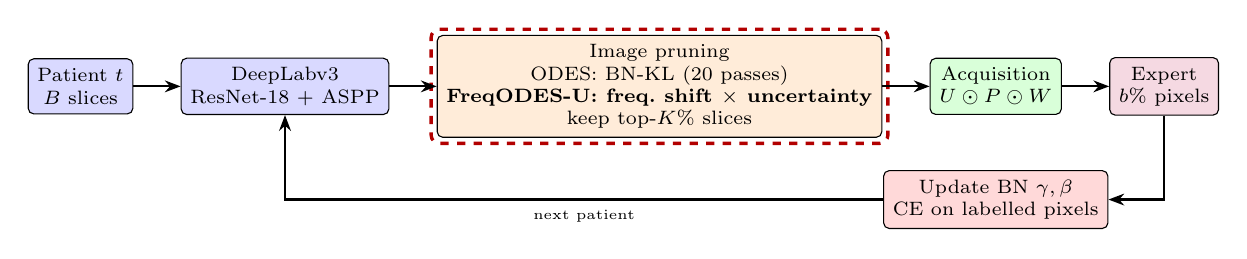
\begin{tikzpicture}[node distance=4mm and 6mm]
  \node[blk=blue] (in) {Patient $t$\\$B$ slices};
  \node[blk=blue, right=of in] (net) {DeepLabv3\\ResNet-18 + ASPP};
  \node[blk=orange, right=of net] (prune) {Image pruning\\ODES: BN-KL (20 passes)\\\textbf{FreqODES-U: freq.\ shift $\times$ uncertainty}\\keep top-$K\%$ slices};
  \node[blk=green, right=of prune] (acq) {Acquisition\\$U\odot P\odot W$};
  \node[blk=purple, right=of acq] (exp) {Expert\\$b\%$ pixels};
  \node[blk=red, below=7mm of acq] (upd) {Update BN $\gamma,\beta$\\CE on labelled pixels};
  \draw[arr] (in) -- (net); \draw[arr] (net) -- (prune); \draw[arr] (prune) -- (acq); \draw[arr] (acq) -- (exp);
  \draw[arr] (exp) |- (upd); \draw[arr] (upd) -| node[pos=0.25,below,font=\tiny]{next patient} (net);
  \begin{scope}[on background layer]\node[new, fit=(prune), inner sep=2pt] {};\end{scope}
\end{tikzpicture}
\caption{Online pipeline for one incoming patient. ODES and FreqODES differ only in the dashed image-pruning block; inference, acquisition and the BN update are identical.}
\label{fig:arch}
\end{figure*}

%=====================================================================
\section{Method: FreqODES}\label{sec:method}
%=====================================================================
\subsection{Why in-phase and out-of-phase images differ in frequency}
T1-DUAL imaging acquires two gradient echoes at echo times at which fat and water protons precess in phase and out of phase. In the IP image the fat and water signals add; in the OOP image they subtract. Voxels that contain both tissues, such as those at organ boundaries surrounded by fat, therefore lose signal in the OOP image and form thin dark contours, the chemical-shift artefact of the second kind. Fatty infiltration of the liver produces a similar, more diffuse signal drop. These changes leave the anatomy unchanged but add sharp, thin intensity transitions and alter local texture, which moves energy from low to high spatial frequencies. A descriptor of how image energy is distributed over spatial frequencies should therefore separate IP from OOP slices without any knowledge of the segmentation network. This physical argument motivates the descriptors below, and Section~\ref{sec:results} confirms it empirically.

\subsection{Frequency-domain shift score}
For a slice $x$ (zero-mean), the \textbf{FFT descriptor} is the vector of log relative energies of $|\mathcal{F}(x)|^2$ in $N_b=16$ concentric radial bands of the centred spectrum. The \textbf{DWT descriptor} is the vector of log relative energies of the sub-bands of a three-level Haar decomposition (LL$_3$ and LH$_l$, HL$_l$, HH$_l$ for $l=1,2,3$). Relative energies remove global brightness and contrast, and the logarithm balances the small high-frequency bands against the large low-frequency band. A reference mean $\mu_f$ and standard deviation $\sigma_f$ of each component are estimated once from 200 random source slices. The shift of a target slice is the diagonal Mahalanobis distance
\begin{equation}
D_{freq}(x)=\frac{1}{d}\sum_{f=1}^{d}\left(\frac{\phi_f(x)-\mu_f}{\sigma_f}\right)^2 ,
\end{equation}
computed for FFT, DWT or their average (FFT+DWT). The score needs no network forward pass, and the descriptor behind each selection can be plotted. We also test a fused score $D=\lambda\hat D_{BN}+(1-\lambda)\hat D_{freq}$, where hats denote normalisation by the batch maximum and $\lambda=1$ recovers ODES. We call the selection by $D_{freq}$ alone \emph{FreqODES v1}.

\subsection{FreqODES-U: frequency shift times uncertainty}
The first evaluation (Section~\ref{sec:v1}) showed that the most frequency-shifted slices are not always the most useful to label. Before running further experiments we therefore designed a second score that also asks whether the model is struggling, $\hat D_{freq}\times\hat A\times\hat H$, where $\hat A$ is the fraction of the slice predicted as organ and $\hat H$ the mean pixel entropy of the softmax prediction, together with the two ablations that drop one factor each. The variant
\begin{equation}
S(x_j)=\hat D_{freq}(x_j)\cdot\hat H(x_j),
\end{equation}
which we call \textbf{FreqODES-U}, performed best. $\hat H$ is computed from the inference prediction that ODES already makes, so the score still needs no additional forward pass. All variants were evaluated with three seeds and are reported in full. Algorithm~\ref{alg:freqodes} summarises one online step.

The two factors play complementary roles. $\hat D_{freq}$ is a property of the image alone: it is high for slices whose appearance is far from the source domain, whether or not the network handles them well. $\hat H$ is a property of the network on that slice: it is high where the current model is unsure, including regions where it is unsure for reasons unrelated to the domain shift, such as small or ambiguous organs. Their product is high only for slices that are both shifted and uncertain, which are the slices on which an expert label is most likely to correct a shift-induced error. Because both factors are normalised by their batch maximum, the score is a relative ranking within each patient and needs no tuning of thresholds.

\begin{algorithm}[t]
\caption{One online step of FreqODES-U for patient $t$}
\label{alg:freqodes}
\begin{algorithmic}[1]
\Require model $f_\theta$; source reference $(\mu_f,\sigma_f)$; budgets $K$, $b$
\State $P_j\gets f_\theta(x_j^t)$ for all slices $j=1,\dots,B_t$ \Comment{inference, also the output}
\For{$j=1$ to $B_t$}
  \State $\phi(x_j^t)\gets$ [FFT band energies, Haar DWT sub-band energies]
  \State $D_j\gets\frac1d\sum_f\big((\phi_f(x_j^t)-\mu_f)/\sigma_f\big)^2$ \Comment{no forward pass}
  \State $H_j\gets$ mean pixel entropy of $P_j$
\EndFor
\State $S_j\gets (D_j/\max_k D_k)\cdot(H_j/\max_k H_k)$
\State $\mathcal{K}_t\gets$ top-$\lceil K B_t\rceil$ slices by $S_j$
\For{each slice in $\mathcal{K}_t$}
  \State select $5\times5$ patches by $U\odot P\odot W$ up to $b$ of the area \Comment{as in ODES}
  \State obtain expert labels for the selected patches
\EndFor
\State update BN parameters $(\gamma,\beta)$ with one Adam step on the labelled pixels
\end{algorithmic}
\end{algorithm}

\subsection{Computational cost}
For a patient with $B$ slices, the ODES score passes $N_{aug}=20$ augmented copies of every slice through a copy of the network, that is $N_{aug}B$ additional forward passes; for a typical CHAOS patient with $B\approx32$ this is about 640 forward passes, about twenty times the cost of segmenting the patient. The frequency descriptor needs one 2-D FFT ($O(HW\log HW)$) and one three-level Haar transform ($O(HW)$) per slice, which takes a few milliseconds on a CPU, and the uncertainty term reuses the inference output. Selection with FreqODES-U is therefore essentially free, and the remaining cost of an online step is dominated by inference, patch acquisition and the BN update. The measured end-to-end times are reported in Section~\ref{sec:cost}.

\subsection{Design choices}
The descriptor uses $N_b=16$ radial bands, which resolve the spectrum of a $256\times256$ slice finely enough to separate low-, mid- and high-frequency energy while keeping each band estimate stable. The Haar wavelet is the simplest orthogonal wavelet; three levels reduce the approximation band to $32\times32$ pixels, the scale of the kidneys and spleen. The reference statistics come from only 200 random source slices, so the score can be prepared once before deployment and the source data are not needed afterwards, as required in the source-free online setting. The diagonal Mahalanobis distance treats each band separately and needs no assumption about the distribution of network activations.

%=====================================================================
\section{Experimental setup}
%=====================================================================
\subsection{Dataset and protocol}
We use the 20 MR training cases of CHAOS~\cite{kavur2021chaos}, T1-DUAL sequence: 647 axial slices (26--50 per patient) of $256\times256$ or $288\times288$ pixels, resized to $256\times256$ and normalised per slice. Labels are liver, right kidney, left kidney and spleen, plus background. Following ODES~\cite{islam2025odes}, the source model is trained on the IP volumes, and the 20 OOP volumes are streamed once, in a fixed order, as 20 online batches. Each patient is evaluated right after its own adaptation step. Table~\ref{tab:data} summarises the data. The classes are strongly imbalanced: background covers 95.5\% of the pixels and each kidney less than 0.4\%, which explains why the kidneys are the most sensitive organs to domain shift and why we report per-organ results.

\begin{table}[t]
\caption{CHAOS T1-DUAL data used in this study. Pixel shares are computed over all 647 slices.}
\label{tab:data}
\centering\small
\begin{tabular}{ll}
\toprule
Property & Value \\
\midrule
Patients & 20 (CHAOS MR training set) \\
Sequences & T1-DUAL in-phase (source), out-of-phase (target) \\
Slices per patient & 26--50 (647 in total) \\
In-plane size & $256\times256$ or $288\times288$ $\rightarrow$ $256\times256$ \\
Liver pixels & 3.21\% \\
Right / left kidney pixels & 0.35\% / 0.36\% \\
Spleen pixels & 0.56\% \\
Background pixels & 95.52\% \\
\bottomrule
\end{tabular}
\end{table}

\subsection{Completing the ODES implementation}
Our implementation is built on the official ODES code released by its authors (\url{https://github.com/ShazidAraf/ODES}), which provides the online loop but not a runnable pipeline. We added a CHAOS conversion script (checking slice--label alignment), a source-training script, and the module \texttt{FFT\_weight\_2.py}, which the code imports but which was not released; we re-implemented it from Algorithm~2 of~\cite{islam2025odes}. We also removed hard-coded GPU calls, enabled the diversity map (its multiplication was commented out) and fixed a stale variable through which a previous slice's acquisition map could be used.

\subsection{Implementation details}
The segmentation network is DeepLabv3 with an ImageNet-initialised ResNet-18 encoder and an ASPP module (16.6\,M parameters), as in ODES. It is trained on IP slices for 25 epochs with Adam (learning rate $10^{-3}$, weight decay $10^{-4}$, cosine schedule), batch size 8, cross-entropy plus Dice loss, and flips, $90^\circ$ rotations and intensity jitter. Online adaptation uses Adam with learning rate $10^{-2}$ and one step per patient, updating only the 13{,}792 BN affine parameters. The pixel budget is $b=1\%$ (26 patches of $5\times5$ pixels per selected slice) and the slice budget is $K\in\{10,50,100\}\%$. The BN-KL score uses 20 augmented copies per slice, as in the released code. All experiments ran in PyTorch on an NVIDIA Tesla T4 GPU. Tables~\ref{tab:hyper} and~\ref{tab:arch} list all settings and the network dimensions; every method uses the same values, so they differ only in the slice-selection score.

\begin{table}[t]
\caption{Hyper-parameters, shared by all methods.}
\label{tab:hyper}
\centering\small
\begin{tabular}{ll}
\toprule
Setting & Value \\
\midrule
\multicolumn{2}{l}{\emph{Source training}} \\
Encoder initialisation & ImageNet ResNet-18 \\
Optimiser, learning rate & Adam, $10^{-3}$, cosine schedule \\
Weight decay, batch size, epochs & $10^{-4}$, 8, 25 \\
Loss & cross-entropy + Dice \\
Augmentation & flips, $90^\circ$ rotations, intensity jitter \\
\multicolumn{2}{l}{\emph{Online adaptation}} \\
Updated parameters & BN $\gamma,\beta$ (13{,}792, 0.08\%) \\
Optimiser, learning rate, steps & Adam, $10^{-2}$, 1 per patient \\
Pixel budget $b$ & 1\% of each selected slice \\
Patch size & $5\times5$ (26 patches per slice) \\
Slice budget $K$ & 10\%, 50\%, 100\% \\
Augmented copies (BN-KL) & 20 \\
Diversity map & threshold 0.5, $\alpha=5$ \\
\multicolumn{2}{l}{\emph{Frequency score}} \\
FFT bands & 16 radial bands \\
Wavelet & Haar, 3 levels (10 sub-bands) \\
Reference set & 200 random source slices \\
Seeds & 12345 (single-seed study); 1, 2, 12345 \\
\bottomrule
\end{tabular}
\end{table}

\begin{table}[t]
\caption{Segmentation network (DeepLabv3, ResNet-18 encoder) for a $3\times256\times256$ input.}
\label{tab:arch}
\centering\small
\begin{tabular}{lrr}
\toprule
Block & Output size & Parameters \\
\midrule
Stem (conv $7\times7$, max-pool) & $64\times64\times64$ & 9.5\,k \\
ResNet layer 1 (low-level feature) & $64\times64\times64$ & 148\,k \\
ResNet layers 2--3 & $256\times16\times16$ & 2.63\,M \\
ResNet layer 4 (high-level feature) & $512\times8\times8$ & 8.39\,M \\
ASPP (rates 6, 12, 18 + pooling) & $256\times8\times8$ & 4.13\,M \\
Decoder (skip $48$ ch., two $3\times3$ convs) & $256\times64\times64$ & 1.29\,M \\
Classifier + $4\times$ upsampling & $5\times256\times256$ & 1.3\,k \\
\midrule
Total & & 16.60\,M \\
\bottomrule
\end{tabular}
\end{table}

\subsection{Evaluation}
We report Dice and Jaccard (IoU) per organ and averaged, and the wall-clock time of a full online pass over the 20 patients. Methods are compared with a paired Wilcoxon signed-rank test on per-patient mean Dice. The first study uses one seed; the FreqODES-U study uses three seeds (1, 2, 12345), giving 60 paired patient-runs per method.

%=====================================================================
\section{Results}\label{sec:results}
%=====================================================================
\subsection{Shift detection}
Fig.~\ref{fig:freq} shows that OOP slices carry systematically more high-frequency energy than IP slices in both descriptors. Using the score alone to separate held-out IP slices from OOP slices gives ROC-AUC values of \AUCFFT\ (FFT), \AUCDWT\ (DWT) and \AUCFREQ\ (FFT+DWT), and the score grows steadily with synthetic noise and blur.

\begin{figure*}[t]
\centering
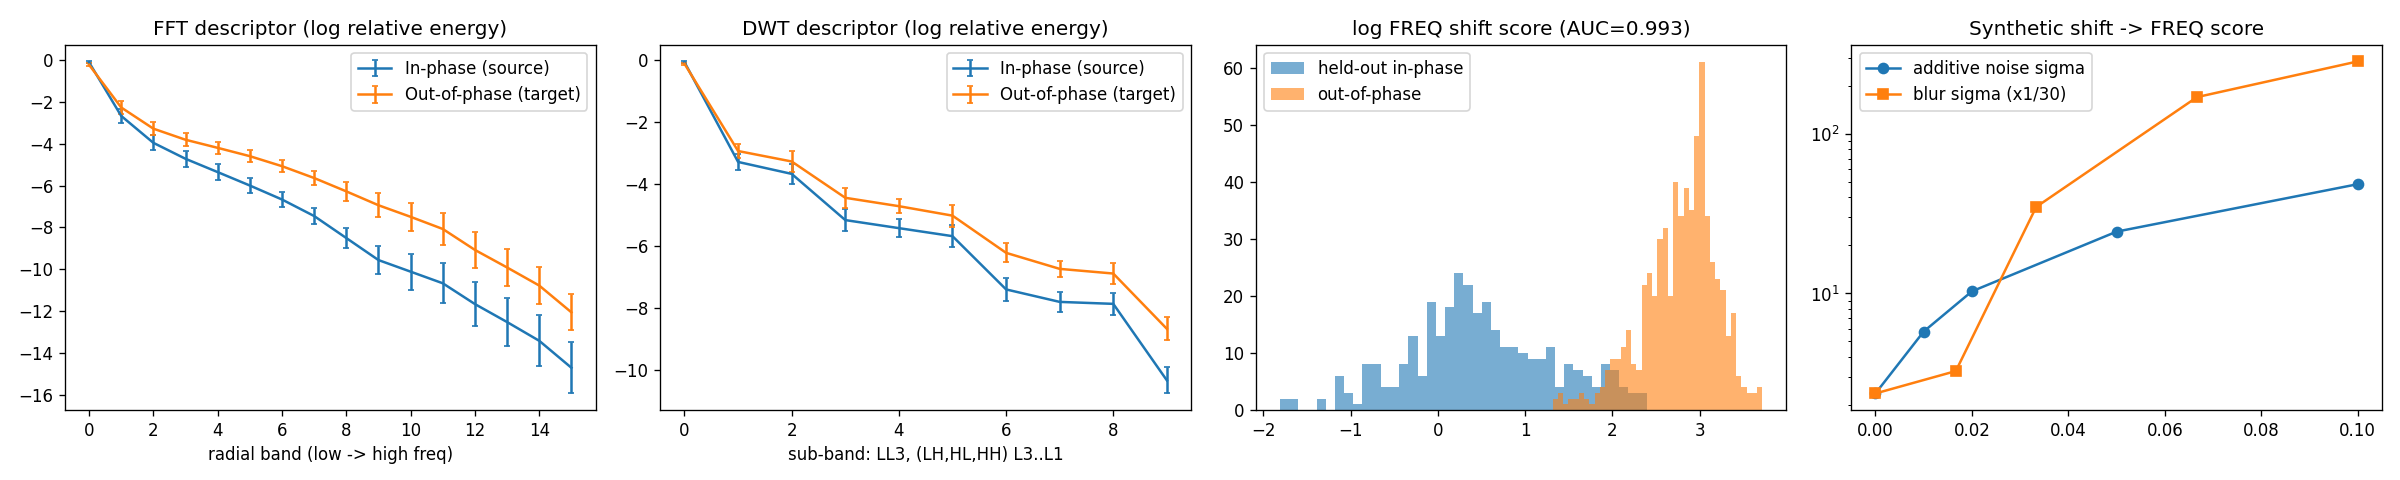
\includegraphics[width=\textwidth]{figures/freq_analysis.png}
\caption{Frequency analysis of CHAOS T1-DUAL. From left: mean FFT radial-band descriptor, mean DWT sub-band descriptor (error bars: standard deviation), histogram of the FFT+DWT shift score, and the score under synthetic noise and blur.}
\label{fig:freq}
\end{figure*}

\subsection{Reproduction of ODES}
Table~\ref{tab:rep} compares our reproduction with the published results. With all slices annotated we obtain \DODESK\% mean Dice (reported: 78.61\%), and the source-only model reaches \Dsourceonly\% (reported: 52.99\%), so the gain of about 25 Dice points from adaptation is reproduced, as is the trend over $K$. No source checkpoint or training recipe is published, so the remaining organ-level differences, notably for the kidneys, most likely come from source training. Fig.~\ref{fig:train} shows the training loss and the per-patient Dice during online adaptation.

\begin{table*}[t]
\caption{Reproduction of ODES on CHAOS IP$\rightarrow$OOP ($b=1\%$, single seed). Dice per organ and mean Dice / Jaccard (\%). Reported values are from Table~1 of~\cite{islam2025odes}, which gives no Jaccard.}
\label{tab:rep}
\centering\small
\begin{tabular}{llcccccc}
\toprule
Setting & Source & Liver & L.\,kidney & R.\,kidney & Spleen & Mean DSC & Mean IoU \\
\midrule
\multirow{2}{*}{Source only} & Reported & 87.77 & 37.97 & 18.92 & 67.31 & 52.99 & -- \\
 & Ours & \DsourceonlyLiver & \DsourceonlyLK & \DsourceonlyRK & \DsourceonlySpleen & \Dsourceonly & \Jsourceonly \\
\multirow{2}{*}{ODES, $K=100\%$} & Reported & 88.90 & 72.41 & 74.55 & 78.56 & 78.61 & -- \\
 & Ours & \DODESKLiver & \DODESKLK & \DODESKRK & \DODESKSpleen & \DODESK & \JODESK \\
\multirow{2}{*}{ODES, $K=50\%$} & Reported & 89.13 & 72.30 & 74.43 & 78.36 & 78.56 & -- \\
 & Ours & \DBNKFiftyLiver & \DBNKFiftyLK & \DBNKFiftyRK & \DBNKFiftySpleen & \DBNKFifty & \JBNKFifty \\
\multirow{2}{*}{ODES, $K=10\%$} & Reported & 88.41 & 71.45 & 70.22 & 77.12 & 76.80 & -- \\
 & Ours & \DBNKTenLiver & \DBNKTenLK & \DBNKTenRK & \DBNKTenSpleen & \DBNKTen & \JBNKTen \\
\bottomrule
\end{tabular}
\end{table*}

\begin{figure*}[t]
\centering
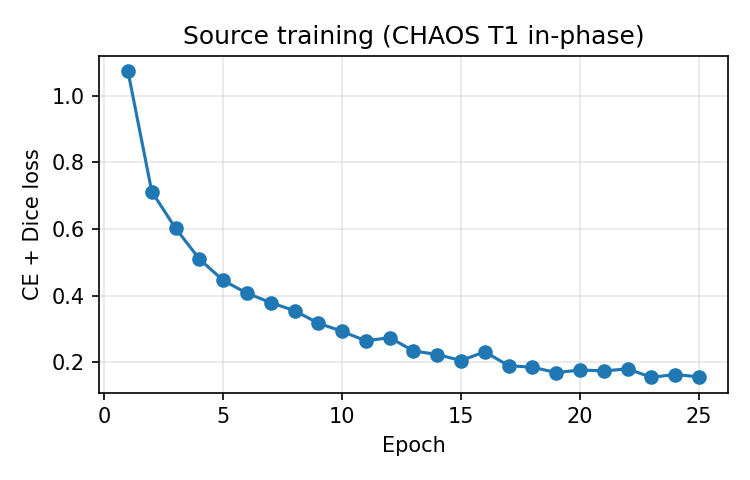
\includegraphics[width=0.38\textwidth]{figures/train_loss.png}\hspace{6mm}
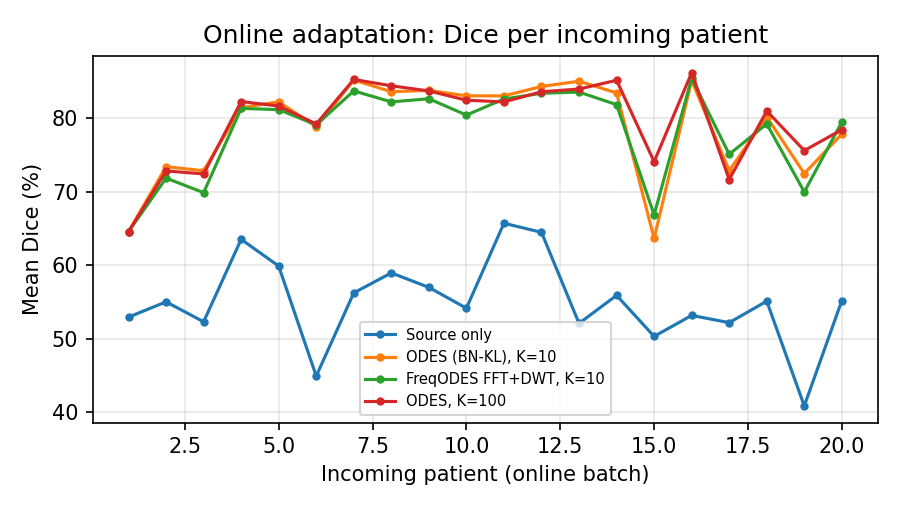
\includegraphics[width=0.48\textwidth]{figures/online_dice.png}
\caption{Left: training loss of the source model on IP slices. Right: mean Dice of each incoming target patient during online adaptation.}
\label{fig:train}
\end{figure*}

\begin{figure*}[t]
\centering
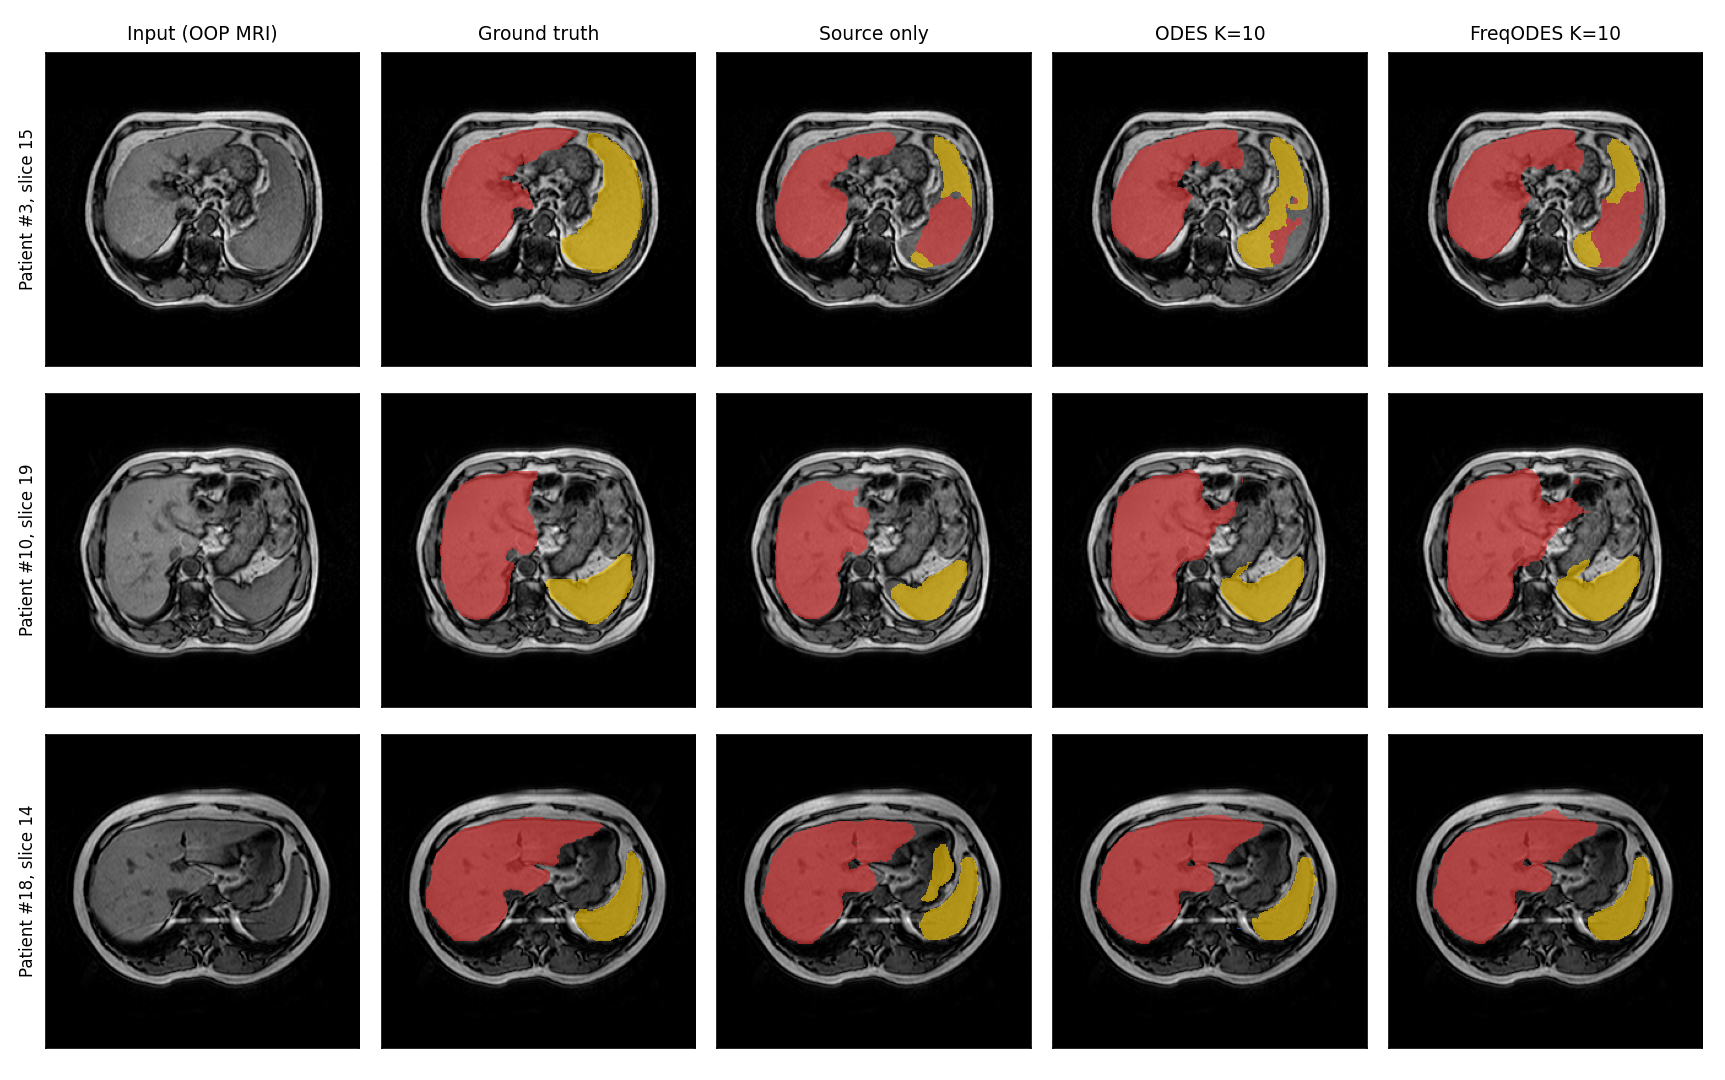
\includegraphics[width=0.9\textwidth]{figures/qualitative.png}
\caption{Qualitative results on three OOP patients: input, ground truth, and the predictions of the source model, ODES ($K=10\%$) and FreqODES v1 ($K=10\%$). Red: liver; green: right kidney; blue: left kidney; yellow: spleen.}
\label{fig:qual}
\end{figure*}

\subsection{Frequency score alone (FreqODES v1)}\label{sec:v1}
Table~\ref{tab:cmp} compares the pruning scores at equal budget in the single-seed study. The pure frequency scores trail ODES by 0.6--0.8 Dice at $K=10\%$ and by 0.3--0.5 at $K=50\%$, while the fused score and random pruning are close to ODES. Frequency pruning shortens the online pass from \TBNKTen\,s to \TFREQKTen\,s. Qualitative results are shown in Fig.~\ref{fig:qual}, and Fig.~\ref{fig:budget} shows Dice as a function of the slice budget.

\begin{table*}[t]
\caption{Single-seed comparison of pruning scores ($b=1\%$). DSC / IoU in \%; $p$: paired Wilcoxon signed-rank test over the 20 patients against ODES at the same $K$; time: full online pass on a T4.}
\label{tab:cmp}
\centering\small
\begin{tabular}{lcccc@{\hskip 5mm}cccc}
\toprule
 & \multicolumn{4}{c}{$K=10\%$} & \multicolumn{4}{c}{$K=50\%$} \\
Pruning score & DSC & IoU & $p$ & Time (s) & DSC & IoU & $p$ & Time (s) \\
\midrule
BN-KL (ODES) & \DBNKTen & \JBNKTen & -- & \TBNKTen & \DBNKFifty & \JBNKFifty & -- & \TBNKFifty \\
FFT & \DFFTKTen & \JFFTKTen & \PFFTKTen & \TFFTKTen & \DFFTKFifty & \JFFTKFifty & \PFFTKFifty & \TFFTKFifty \\
DWT & \DDWTKTen & \JDWTKTen & \PDWTKTen & \TDWTKTen & \DDWTKFifty & \JDWTKFifty & \PDWTKFifty & \TDWTKFifty \\
FFT+DWT & \DFREQKTen & \JFREQKTen & \PFREQKTen & \TFREQKTen & \DFREQKFifty & \JFREQKFifty & \PFREQKFifty & \TFREQKFifty \\
Fused ($\lambda=0.5$) & \DFUSEDKTenLFifty & \JFUSEDKTenLFifty & \PFUSEDKTenLFifty & \TFUSEDKTenLFifty & \DFUSEDKFiftyLFifty & \JFUSEDKFiftyLFifty & \PFUSEDKFiftyLFifty & \TFUSEDKFiftyLFifty \\
Random & \DRANDOMKTen & \JRANDOMKTen & \PRANDOMKTen & \TRANDOMKTen & \DRANDOMKFifty & \JRANDOMKFifty & \PRANDOMKFifty & \TRANDOMKFifty \\
\bottomrule
\end{tabular}
\end{table*}

\begin{figure*}[t]
\centering
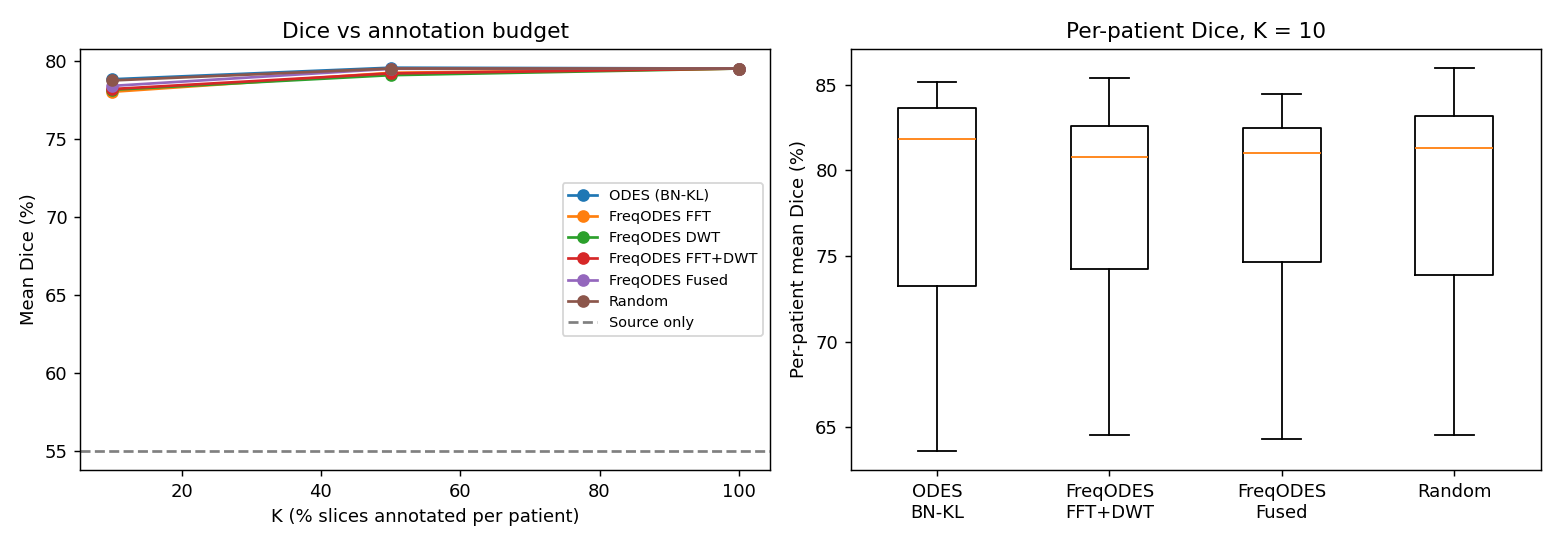
\includegraphics[width=0.85\textwidth]{figures/dice_vs_budget.png}
\caption{Single-seed study. Left: mean Dice versus the share $K$ of slices annotated. Right: per-patient Dice at $K=10\%$.}
\label{fig:budget}
\end{figure*}

\subsection{FreqODES-U over three seeds}
Table~\ref{tab:v2} and Fig.~\ref{fig:v2} report all v2 variants over three seeds. With 10\% of slices annotated, FreqODES-U reaches \VFeTenMean\% mean Dice against \VBnTenMean\% for ODES ($\Delta=\VFeTenDiff$, $p=\VFeTenP$ over 60 paired patient-runs), and it is better on every seed (\VFeTenSa, \VFeTenSb, \VFeTenSc\ vs.\ \VBnTenSa, \VBnTenSb, \VBnTenSc). It is also far more stable across seeds (standard deviation \VFeTenStd\ vs.\ \VBnTenStd) and about one third faster. The planned v2 score with the organ-area term (\VFvTenMean\%) and the area-only ablation (\VFaTenMean\%) are not significantly different from ODES. With 50\% of slices annotated, ODES remains best (\VBnFiftyMean\% vs.\ \VFeFiftyMean\%, $p=\VFeFiftyP$). The single-seed numbers of Section~\ref{sec:v1} differ from these averages by up to about one Dice point, which shows why several seeds are needed for differences of this size.

\begin{table*}[t]
\caption{FreqODES-U and its variants over three seeds. Mean Dice $\pm$ standard deviation (\%); $\Delta$ and $p$: paired Wilcoxon signed-rank test against ODES over 60 patient-runs; time: full online pass on a T4.}
\label{tab:v2}
\centering\small
\begin{tabular}{lcccc@{\hskip 5mm}ccc}
\toprule
 & \multicolumn{4}{c}{$K=10\%$} & \multicolumn{3}{c}{$K=50\%$} \\
Selection score & DSC & $\Delta$ / $p$ & IoU & Time (s) & DSC & $\Delta$ / $p$ & IoU \\
\midrule
ODES (BN-KL)~\cite{islam2025odes} & \VBnTenMean$\pm$\VBnTenStd & -- & \VBnTenIoU & \VBnTenTime & \VBnFiftyMean$\pm$\VBnFiftyStd & -- & \VBnFiftyIoU \\
v1: frequency & \VFqTenMean$\pm$\VFqTenStd & \VFqTenDiff\ / \VFqTenP & \VFqTenIoU & \VFqTenTime & \VFqFiftyMean$\pm$\VFqFiftyStd & \VFqFiftyDiff\ / \VFqFiftyP & \VFqFiftyIoU \\
v2: freq.\ $\times$ area $\times$ unc. & \VFvTenMean$\pm$\VFvTenStd & \VFvTenDiff\ / \VFvTenP & \VFvTenIoU & \VFvTenTime & \VFvFiftyMean$\pm$\VFvFiftyStd & \VFvFiftyDiff\ / \VFvFiftyP & \VFvFiftyIoU \\
freq.\ $\times$ area & \VFaTenMean$\pm$\VFaTenStd & \VFaTenDiff\ / \VFaTenP & \VFaTenIoU & \VFaTenTime & -- & -- & -- \\
\textbf{FreqODES-U} & \textbf{\VFeTenMean}$\pm$\VFeTenStd & \VFeTenDiff\ / \VFeTenP & \VFeTenIoU & \VFeTenTime & \VFeFiftyMean$\pm$\VFeFiftyStd & \VFeFiftyDiff\ / \VFeFiftyP & \VFeFiftyIoU \\
Random & \VRdTenMean$\pm$\VRdTenStd & \VRdTenDiff\ / \VRdTenP & \VRdTenIoU & \VRdTenTime & \VRdFiftyMean$\pm$\VRdFiftyStd & \VRdFiftyDiff\ / \VRdFiftyP & \VRdFiftyIoU \\
\bottomrule
\end{tabular}
\end{table*}

\begin{figure*}[t]
\centering
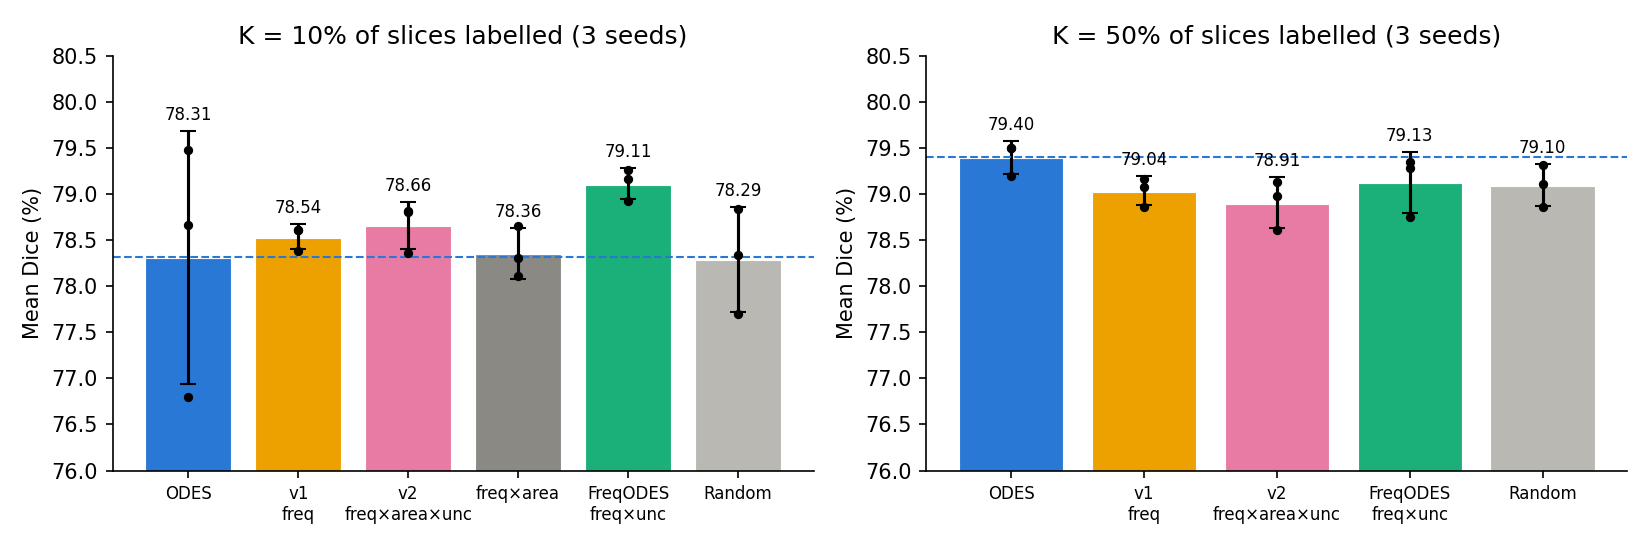
\includegraphics[width=0.9\textwidth]{figures/v2_results.png}
\caption{Three-seed results. Bars: mean Dice; error bars: standard deviation; dots: individual seeds; dashed line: ODES.}
\label{fig:v2}
\end{figure*}

\subsection{Per-organ and per-patient analysis}
Table~\ref{tab:organ} breaks the three-seed results down by organ. At $K=10\%$ the gain of FreqODES-U comes from the small organs: the left kidney improves from \VBnTenLK\% to \VFeTenLK\%, the right kidney from \VBnTenRK\% to \VFeTenRK\% and the spleen from \VBnTenSpleen\% to \VFeTenSpleen\%, while the liver, which is large and already well segmented, is unchanged (\VBnTenLiver\% vs.\ \VFeTenLiver\%). This matches the design of the score: the entropy factor is highest around small, uncertain structures, so the selected slices tend to contain kidneys and spleen, and the expert's patches correct exactly the organs that suffer most from the shift. The frequency score alone (v1) improves the left kidney (\VFqTenLK\%) and the spleen (\VFqTenSpleen\%) over ODES but not the right kidney (\VFqTenRK\%); adding the uncertainty factor lifts both kidneys.

At the patient level, FreqODES-U is better than ODES on \VFeTenWins\ of the 60 patient-runs at $K=10\%$, against \VFqTenWins\ of 60 for the frequency score alone. At $K=50\%$ it is better on \VFeFiftyWins\ of 60, consistent with the small overall advantage of ODES at that budget. The improvement at $K=10\%$ is therefore not caused by a few patients with large gains but is spread over most of the stream.

\begin{table*}[t]
\caption{Per-organ results over three seeds (mean Dice / mean IoU, \%).}
\label{tab:organ}
\centering\small
\begin{tabular}{llcccc}
\toprule
$K$ & Selection score & Liver & Left kidney & Right kidney & Spleen \\
\midrule
\multirow{3}{*}{10\%} & ODES (BN-KL) & \VBnTenLiver\ / \VBnTenLiverJ & \VBnTenLK\ / \VBnTenLKJ & \VBnTenRK\ / \VBnTenRKJ & \VBnTenSpleen\ / \VBnTenSpleenJ \\
 & v1: frequency & \VFqTenLiver\ / \VFqTenLiverJ & \VFqTenLK\ / \VFqTenLKJ & \VFqTenRK\ / \VFqTenRKJ & \VFqTenSpleen\ / \VFqTenSpleenJ \\
 & \textbf{FreqODES-U} & \VFeTenLiver\ / \VFeTenLiverJ & \textbf{\VFeTenLK}\ / \VFeTenLKJ & \textbf{\VFeTenRK}\ / \VFeTenRKJ & \textbf{\VFeTenSpleen}\ / \VFeTenSpleenJ \\
\midrule
\multirow{3}{*}{50\%} & ODES (BN-KL) & \VBnFiftyLiver\ / \VBnFiftyLiverJ & \VBnFiftyLK\ / \VBnFiftyLKJ & \VBnFiftyRK\ / \VBnFiftyRKJ & \VBnFiftySpleen\ / \VBnFiftySpleenJ \\
 & v1: frequency & \VFqFiftyLiver\ / \VFqFiftyLiverJ & \VFqFiftyLK\ / \VFqFiftyLKJ & \VFqFiftyRK\ / \VFqFiftyRKJ & \VFqFiftySpleen\ / \VFqFiftySpleenJ \\
 & FreqODES-U & \VFeFiftyLiver\ / \VFeFiftyLiverJ & \VFeFiftyLK\ / \VFeFiftyLKJ & \VFeFiftyRK\ / \VFeFiftyRKJ & \VFeFiftySpleen\ / \VFeFiftySpleenJ \\
\bottomrule
\end{tabular}
\end{table*}

\subsection{Computational cost}\label{sec:cost}
Fig.~\ref{fig:runtime} shows the wall-clock time of a full online pass over the 20 patients at $K=10\%$ in the single-seed study. Every frequency-based selection runs in \TFFTKTen--\TFREQKTen\,s, close to random selection (\TRANDOMKTen\,s), whereas the BN-KL score of ODES needs \TBNKTen\,s because of its augmented forward passes. Over the three-seed study the averages are \VFeTenTime\,s for FreqODES-U and \VBnTenTime\,s for ODES. The fused scores inherit the cost of the BN term. Because the frequency descriptors can be computed on a CPU while the GPU segments the previous slice, the selection step adds practically no latency to the clinical workflow.

\begin{figure}[t]
\centering
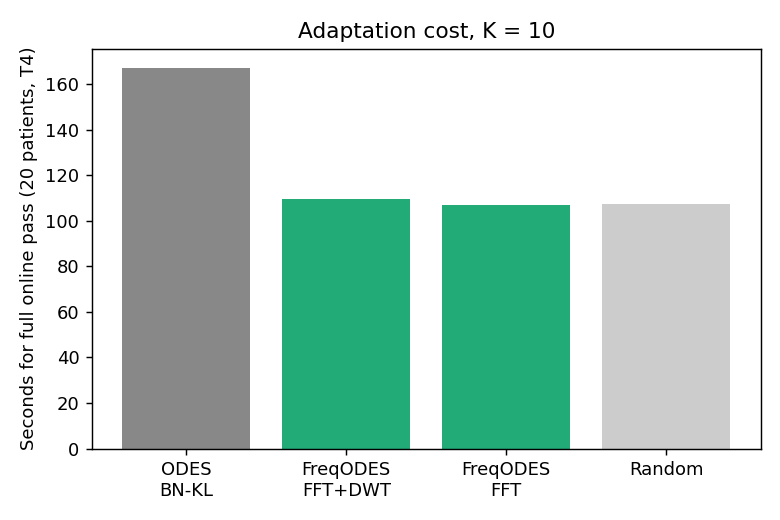
\includegraphics[width=\columnwidth]{figures/runtime.png}
\caption{Wall-clock time of a full online pass over the 20 target patients ($K=10\%$, NVIDIA T4).}
\label{fig:runtime}
\end{figure}

\subsection{Ablation studies}
Table~\ref{tab:abl} reports the pruning $\times$ diversity-weighting ablation of Table~3 in~\cite{islam2025odes} and the fusion-weight sweep, both from the single-seed study. Diversity weighting changes the mean Dice by at most 0.2 points in our runs, much less than the gains reported by ODES. In the fusion sweep the pure frequency score is lowest, and any amount of BN information brings the result back to the level of ODES.

\begin{table}[t]
\caption{Single-seed ablations at $K=10\%$ (mean Dice, \%). Top: image pruning $\times$ diversity weighting (D.W.). Bottom: fusion weight $\lambda$.}
\label{tab:abl}
\centering\small
\begin{tabular}{lcc}
\toprule
Pruning & D.W.\ off & D.W.\ on \\
\midrule
BN-KL (ODES) & \DBNKTennoDW & \DBNKTen \\
FFT+DWT (ours) & \DFREQKTennoDW & \DFREQKTen \\
Random & \DRANDOMKTennoDW & \DRANDOMKTen \\
Reported~\cite{islam2025odes}: BN / random & 75.88 / 74.32 & 76.80 / 75.41 \\
\bottomrule
\end{tabular}\\[3mm]
\begin{tabular}{lc}
\toprule
$\lambda$ & Mean DSC \\
\midrule
0 (frequency only) & \DFREQKTen \\
0.25 & \DFUSEDKTenLQuarter \\
0.5 & \DFUSEDKTenLFifty \\
0.75 & \DFUSEDKTenLThreeQ \\
1 (BN only = ODES) & \DBNKTen \\
\bottomrule
\end{tabular}
\end{table}

%=====================================================================
\section{Discussion}
%=====================================================================
\paragraph{Why the shift score alone is not enough.} The frequency score answers ``how different is this slice from the source?'', whereas slice selection should answer ``which labels will most improve the model?''. The slices with the most unusual spectra are often at the ends of the volume, where organs are small or absent, so labelling them teaches the BN layers little. The BN score of ODES measures what the \emph{network} finds unusual, which is closer to its errors. In addition, the IP$\rightarrow$OOP change affects every slice, so nearly all target slices look shifted and the useful information lies in the ranking among them. This also explains why random selection is competitive, in contrast to the ablation in~\cite{islam2025odes}.

\paragraph{Why FreqODES-U works.} Weighting the shift by the model's uncertainty keeps the cheap, interpretable image-level signal but favours slices on which the network is actually unsure. This agrees with active domain adaptation work that combines domain cues with uncertainty~\cite{xie2022ripu,safaei2025certainty,huynh2026category}, and with continual TTA methods that use uncertainty to stabilise adaptation~\cite{zhu2025uncertainty}. The organ-area term did not help, which suggests that uncertainty already captures what makes a slice informative. At the 50\% budget half of each volume is labelled anyway, so the selection matters less, which is consistent with ODES keeping a small lead there. The lower seed-to-seed variance of FreqODES-U is useful in practice, because an online system cannot re-run a patient.

\paragraph{Interpretability.} A selection made by FreqODES-U can be explained with two quantities that a clinician or engineer can inspect: the radial spectrum or wavelet energies of the slice compared with the source reference (Fig.~\ref{fig:freq}), and the entropy map of the current prediction. The BN-KL score of ODES is a sum of divergences over hundreds of channels in the last nine BN layers, which has no direct visual meaning. In a clinical deployment, an explainable reason for asking an expert to annotate a particular slice makes the request easier to trust and to audit.

\paragraph{Implications for deployment.} Three practical properties follow from the results. First, the selection step costs almost nothing, so it fits within the turnover time even on modest hardware. Second, the seed-to-seed standard deviation of FreqODES-U at $K=10\%$ is about eight times smaller than that of ODES, so the quality delivered to each patient depends less on chance; an online system cannot re-run a patient, so this stability matters as much as the mean. Third, the benefit is largest at the smallest budget, where expert time is scarcest. When a larger budget is available, the advantage disappears and the original BN-based score is slightly better, so the choice of score can follow the available annotation time.

\paragraph{Relation to recent methods.} Recent continual TTA methods improve unsupervised adaptation through prompts~\cite{chen2024vptta,li2025mgipt,du2026spegc}, anchors~\cite{wu2026a3tta}, energy-based shape priors~\cite{zhang2025energy} or foundation models~\cite{ji2026redifm,wu2025samtta}, and recent active adaptation methods refine region selection~\cite{gao2024superpixel,huynh2026category,yan2026tcada}. These directions are complementary to ours: FreqODES-U changes only which slices are shown to the expert, and could be combined with a stronger adaptation step or a finer pixel-acquisition rule. Frequency-domain techniques have so far mostly been used to augment or translate images~\cite{zhao2024morestyle,wu2025randdg,yin2025ddfp}; our results show that the same representation is also useful as a cheap measure of how far each incoming slice lies from the training domain.

\paragraph{Threats to validity.} The reproduction differs from the published ODES numbers by up to two Dice points because the source model had to be retrained; all methods share our source model, so the comparison between selection scores is unaffected. The online stream follows one fixed patient order, and the order may influence online methods. Experts are simulated with ground-truth labels, so annotation noise and annotation time are not modelled. Finally, the IP$\rightarrow$OOP shift is global and comparatively mild; the conclusions may change for shifts that vary strongly between slices or patients.

\paragraph{Limitations.} FreqODES-U was the best variant of a pre-planned ablation rather than the planned score itself, so its advantage should be confirmed on further data; we report every variant to make this transparent. The evaluation uses one adaptation pair, 20 patients and three seeds, and the expert is simulated with ground-truth labels. Future work includes the CHAOS$\rightarrow$DUKE and BMC$\rightarrow$RUNMC scenarios of~\cite{islam2025odes}, more seeds and stream orders, spectra computed inside organ regions of interest, and combining the score with recent prompt-based and foundation-model TTA methods~\cite{li2025mgipt,ji2026redifm,du2026spegc}.

%=====================================================================
\section{Conclusion}
%=====================================================================
Building on ODES~\cite{islam2025odes}, we reproduced online expert-guided domain adaptation on CHAOS T1-DUAL IP$\rightarrow$OOP after completing its public implementation, and studied how slices should be selected for expert annotation. A Fourier and wavelet shift score detects the domain shift almost perfectly and without any forward pass, but shift magnitude alone is an incomplete proxy for annotation value. Combining it with the model's uncertainty, FreqODES-U outperforms ODES when only 10\% of slices are annotated (\VFeTenMean\% vs.\ \VBnTenMean\% Dice over three seeds, $p=\VFeTenP$), with lower variance and about one third less computation, while ODES stays slightly better at a 50\% budget.

\section*{Data and code availability}
Code, configuration, logs and result files are available at \url{https://github.com/Vishnu868/FreqODES}. It extends the official ODES implementation~\cite{islam2025odes} (\url{https://github.com/ShazidAraf/ODES}), distributed under the UCR Academic Software License. The CHAOS dataset~\cite{kavur2021chaos} is available from Zenodo (record 3431873).

\section*{CRediT authorship contribution statement}
\textbf{Vishnu Vardhan:} Software, Data curation, Investigation, Methodology. \textbf{Nithya Sai:} Conceptualization, Formal analysis, Validation, Visualization, Writing -- original draft. Both authors: Writing -- review \& editing.

\section*{Declaration of competing interest}
The authors declare that they have no known competing financial interests or personal relationships that could have appeared to influence the work reported in this paper.

\section*{Acknowledgement}
The ODES software used in this research was created by Amit Roy-Chowdhury and members of the Vision and Learning Group at UCR. \copyright\ 2025 UCR.

\bibliographystyle{cas-model2-names}
\bibliography{refs}

\end{document}
